\chapter{Metodologia}

\section{Parâmetros geométricos e sistemas de coordenadas}

Seja $(x, y, z)$ um ponto referido à um sistema de coordenadas Cartesianas com eixo $x$ apontado para o norte, $y$ para leste e $z$ para baixo. Por conveniência, este sistema de coordenadas foi denominado \textit{sistema de coordenadas principal}.
Considerando um corpo elipsoidal com centro no ponto $(x_{c}, y_{c}, z_{c})$, semi-eixos definidos por constantes positivas $a$, $b$, $c$ e orientações definidas por três ângulos $\varepsilon$, $\zeta$, e $\eta$ (Figura \ref{fig:structural_orientation_angles}). Os ângulos $\varepsilon$, $\zeta$, e $\eta$ são chamados \textit{strike}, \textit{dip} e \textit{rake}, respectivamente, e são comumente usados para definir a orientação de estruturas geológicas\citep{clark1986, allmendinger2012}. 

Os pontos localizados sobre a superfície deste corpo elipsoidal satisfazem a seguinte equação:
\begin{equation}
(\mathbf{r} - \mathbf{r}_c)^T \mathbf{A} (\mathbf{r} - \mathbf{r}_c) = 1 \: ,
\label{eq:ellipsoid_surface}
\end{equation}
em que $\mathbf{r} = [\begin{array}{ccc} x & y & z \end{array} ]^{\top}$,
$\mathbf{r}_{c} = [\begin{array}{ccc} x_{c} & y_{c} & z_{c} \end{array} ]^{\top}$,
$\mathbf{A}$ é uma matriz positiva definida dada por:
\begin{equation}
\mathbf{A} = \mathbf{V}
\left[ \begin{array}{ccc}
a^{-2} & 0 & 0 \\
0 & b^{-2} & 0 \\
0 & 0 & c^{-2} 
\end{array} \right] \mathbf{V}^{\top} \: ,
\label{eq:A}
\end{equation}
e $\mathbf{V}$ é uma matriz ortogonal cujas colunas são definidas por vetores unitários $\mathbf{v}_{1}$, $\mathbf{v}_{2}$, e $\mathbf{v}_{3}$ (Fig. \ref{fig:structural_orientation_angles}b), respectivamente. Estes vetores unitários são comumente descritos em termos de ângulos auxiliares $\alpha$, $\gamma$, e $\delta$, que não são usados pela comunidade geocientífica. Entretanto podemos defini-los a partir de $\varepsilon$, $\zeta$, e $\eta$ como dado por \citep{clark1986}:

\begin{equation}
\alpha = \varepsilon - \cos^{-1} \left[ \frac{\cos \eta}
{\left( 1 - \sin^{2} \zeta \, \sin^{2} \eta \right)^{\frac{1}{2}}}\right] \: ,
\label{eq:alpha}
\end{equation}
\begin{equation}
\gamma = \tan^{-1} \left( \frac{\cos \zeta}{\sin \zeta \, \cos \eta}\right)
\label{eq:gamma}
\end{equation}
e
\begin{equation}
\delta = \sin^{-1} \left( \sin \zeta \, \sin \eta \right) \: ,
\label{eq:delta}
\end{equation}
em que $-90^{\circ} \leq \gamma \leq 90^{\circ}$ e $0 \leq \delta \leq 90^{\circ}$. Assim, dados os ângulos $\varepsilon$, $\zeta$, e $\eta$ (Fig. \ref{fig:structural_orientation_angles}a e Eqs. \ref{eq:alpha}, \ref{eq:gamma}, e
\ref{eq:delta}), podemos definir os vetores unitários
$\mathbf{v}_{1}$, $\mathbf{v}_{2}$, e $\mathbf{v}_{3}$
(Fig. \ref{fig:structural_orientation_angles}b) de acordo com o tipo de elipsoide.
Para elipsoides triaxiais (i.e., $a > b > c$), estes vetores unitários são dados por \citep{clark1986}:

\begin{equation}
\mathbf{v}_{1} = \left[\begin{array}{c} 
-\cos\alpha \; \cos\delta \\
-\sin\alpha \; \cos\delta \\
-\sin\delta
\end{array} \right] \: ,
\label{eq:v1_triaxial_prolate}
\end{equation}
\begin{equation}
\mathbf{v}_{2} = \left[\begin{array}{c} 
\cos\alpha \; \cos\gamma \; \sin\delta + \sin\alpha \; \sin\gamma \\                   
\sin\alpha \; \cos\gamma \; \sin\delta - \cos\alpha \; \sin\gamma \\ 
-\cos\gamma \; \cos\delta
\end{array} \right] \: ,
\label{eq:v2_triaxial_prolate}
\end{equation}                   
\begin{equation}                    
\mathbf{v}_{3} = \left[\begin{array}{c} 
\sin\alpha \; \cos\gamma - \cos\alpha \; \sin\gamma \; \sin\delta \\                    
-\cos\alpha \; \cos\gamma - \sin\alpha \; \sin\gamma \; \sin\delta \\
\sin\gamma \; \cos\delta
\end{array} \right] \: .
\label{eq:v3_triaxial_prolate}
\end{equation}
Similarmente, os vetores unitários $\mathbf{v}_{1}$, $\mathbf{v}_{2}$ e $\mathbf{v}_{3}$ para elipsoides prolatos (i.e., $a > b = c$) são calculados de acordo com as Eqs.
\ref{eq:v1_triaxial_prolate}, \ref{eq:v2_triaxial_prolate}, e
\ref{eq:v3_triaxial_prolate}, mas com $\gamma = 0^{\circ}$ 
\citep{emerson1985}.

Finalmente, os vetores unitários $\mathbf{v}_{1}$, $\mathbf{v}_{2}$ e $\mathbf{v}_{3}$ para elipsoides oblatos (i.e., $a < b = c$) são calculados da seguinte forma:
\begin{equation}
\mathbf{v}_{1} = \left[\begin{array}{c} 
-\cos\alpha \; \sin\gamma \; \sin\delta + \sin\alpha \; \cos\gamma \\               
-\sin\alpha \; \sin\gamma \; \sin\delta - \cos\alpha \; \cos\gamma \\ 
\sin\gamma \; \cos\delta
\end{array} \right] \: ,
\label{eq:v1_oblate}
\end{equation}
\begin{equation}
\mathbf{v}_{2} = \left[\begin{array}{c} 
-\cos\alpha \; \cos\delta \\
-\sin\alpha \; \cos\delta \\
-\sin\delta
\end{array} \right] \: ,
\label{eq:v2_oblate}
\end{equation}                   
\begin{equation}                    
\mathbf{v}_{3} = \left[\begin{array}{c} 
\sin\alpha \; \sin\gamma + \cos\alpha \; \cos\gamma \; \sin\delta \\                    
-\cos\alpha \; \sin\gamma + \sin\alpha \; \cos\gamma \; \sin\delta \\
-\cos\gamma \; \cos\delta
\end{array} \right] \: .
\label{eq:v3_oblate}
\end{equation}

Dessa forma, a matriz $\mathbf{V}$ fica definida como:
\begin{equation}
\mathbf{V} = \left[ \begin{array}{ccc}
\mathbf{v}_{1} & \mathbf{v}_{2} & \mathbf{v}_{3}
\end{array} \right] \: .
\label{eq:V_triaxial_prolate}
\end{equation}
em que $\mathbf{v}_{1}$, $\mathbf{v}_{2}$ e $\mathbf{v}_{3}$ são calculados com as Eqs.
\ref{eq:v1_triaxial_prolate}, \ref{eq:v2_triaxial_prolate}, e \ref{eq:v3_triaxial_prolate} dependendo do tipo de elipsoide.

A modelagem magnética de um corpo elipsoidal é comumente feita em um sistema de coordenadas Cartesianas particular, alinhado com os semi-eixos e sua origem coincidente com o centro do elipsoide (Fig. \ref{fig:structural_orientation_angles}b). Por conveniência, este sistema de coordenas foi denominado \textit{sistema de coordenadas local}.
A relação entre as coordenas Cartesianas $(\tilde{x}, \tilde{y}, \tilde{z})$
de um ponto no sistema de coordenadas local e as coordenadas Cartesianas $(x, y, z)$ do mesmo ponto no sistema principal é dada por:
\begin{equation}
\tilde{\mathbf{r}} = \mathbf{V}^{\top} \left( \mathbf{r} - \mathbf{r}_{c} \right) \: ,
\label{eq:coord_transformation}
\end{equation}
em que 
$\tilde{\mathbf{r}} = [\begin{array}{ccc} \tilde{x} & 
\tilde{y} & 
\tilde{z} \end{array} ]^{\top}$,
$\mathbf{r}$ e $\mathbf{r}_{c}$
são definidas na Eq. \ref{eq:ellipsoid_surface} e a matriz $\mathbf{V}$  (Eq. \ref{eq:V_triaxial_prolate})
é definida de acordo com o tipo de elipsoide. Ao longo deste trabalho, as grandezas referidas ao sistema de coordenadas local são representadas utilizando-se símbolo "$\sim$".

\begin{figure}[hbt!]
	\centering 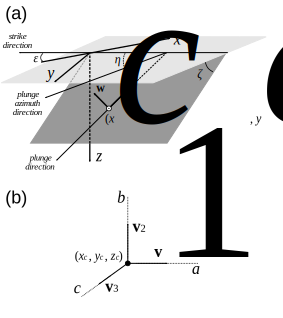
\includegraphics[width=12 cm,height=14.5 cm]{figures/structural_orientation_angles}
	\caption[Esquema representativo do sistema de coordenadas usado para representar um corpo elipsoidal.]{Esquema representativo do sistema de coordenadas usado para representar um corpo elipsoidal. a) Sistema de coordenadas principal com eixo $x$ apontado para norte, $y$ apontado para leste e $z$ para baixo. O plano cinza escuro contém o centro ($x_c$, $y_c$, $z_c$) (círculo branco) e dois vetores unitários, $u$ e $w$, que definem dois semi-eixos do corpo elipsoidal. Para elipsoides triaxiais e prolatos, $u$ e $w$ definem, respectivamente, os semi-eixos $a$ e $b$. Para elipsoides oblatos, $u$ e $w$ definem os semi-eixos $b$ e $a$, respectivamente. A \textit{direção de strike} é definida pela intersecção do plano cinza escuro e o plano horizontal (representado em cinza claro), que contém os eixos $x$ e $y$. O ângulo $\varepsilon$ entre "menos $x$" e a \textit{direção de strike} é chamado de \textit{strike}. O ângulo $\zeta$ entre o plano horizontal e o plano cinza escuro é chamado de \textit{dip}. A linha que contém o vetor unitário $u$ define a \textit{direção de plunge}. O ângulo $\eta$ entre a \textit{direção de strike} e a \textit{direção de plunge} é chamada de \textit{rake}. A projeção da \textit{direção de plunge} no plano horizontal é chamado de \textit{direção azimutal de plunge}. b) Sistema de coordenadas local com origem no centro do elipsoide ($x_c$, $y_c$, $z_c$) (ponto preto) e eixos definidos pelos vetores unitários $v_1$, $v_2$ e $v_3$. Estes vetores unitários definem os semi-eixos $a$, $b$ e $c$ dos elipsoides triaxiais, prolatos e oblatos da mesma forma. Para os  elipsoides triaxiais e prolatos, os vetores unitários $u$ e $w$, mostrados em  (a), coincidem com $v_1$ e $v_2$, respectivamente. Para elipsoides oblatos, os vetores unitários $u$ e $w$, mostrados em (a), coincidem com $v_2$ e $v_3$, respectivamente.}
	\label{fig:structural_orientation_angles}
\end{figure}

\section{Background Teórico}

Considere um corpo geológico localizado na crosta, que possua volume $\vartheta$, formato aproximadamente elipsoidal e que esteja imerso em um campo magnético uniforme $\mathbf{{H}_{0}}$ ($\unit{Am^{-1}}$) dado por:
\begin{equation}
\mathbf{H}_{0} = \| \mathbf{H}_{0} \| \left[
\begin{array}{c}
\cos I \: \cos D \\
\cos I \: \sin D \\
\sin I
\end{array}
\right] \: ,
\label{eq:H0}
\end{equation}
em que $\| \cdot \|$ é a norma Euclidiana e $D$ e $I$ são respectivamente, a declinação e inclinação do campo no sistema de coordenas principal (Fig. \ref{fig:structural_orientation_angles}a). Este campo uniforme representa a componente principal do campo magnético da Terra, que presume ser gerado na núcleo externo líquido da Terra. Ao longo deste trabalho, este campo uniforme é denominado \textit{campo geomagnético local}. Na ausência de correntes de condução, o campo magnético total $\mathbf{H}(\mathbf{r})$ (Eq. \ref{eq:A}) na posição $\mathbf{r}$ (Eq. \ref{eq:coord_transformation}) de um ponto no sistema de coordenadas principal é definido como \citep{sharma1966, eskola1980, reitz1992, sttraton2007}:
\begin{equation}
\mathbf{H}(\mathbf{r}) = \mathbf{H}_{0} - \nabla V(\mathbf{r}) \: ,
\label{eq:H}
\end{equation}
em que o segundo termo é o gradiente negativo do potencial magnético escalar $V(\mathbf{r})$ dado por:
\begin{equation}
V(\mathbf{r}) = -\frac{1}{4\pi} \iiint_{\vartheta} 
\mathbf{M}(\mathbf{r}^{\prime})^{\top} 
\nabla \left(
\frac{1}{\| \mathbf{r} - \mathbf{r}^{\prime} \|}
\right) \, dx^{\prime}dy^{\prime}dz^{\prime} \: .
\label{eq:phi-potential}
\end{equation}
Nesta equação, $\mathbf{r}^{\prime} = [\begin{array}{ccc} 
x^{\prime} & y^{\prime} & z^{\prime} \end{array} ]^{\top}$
é o vetor posição de um ponto localizado dentro do volume $\vartheta$, 
a integral é feita sobre as variáveis $x^{\prime}$, $y^{\prime}$ e 
$z^{\prime}$ e 
$\mathbf{M}(\mathbf{r}^{\prime})$ é o vetor de magnetização
(em $\unit{Am^{-1}}$).
A Eq. \ref{eq:phi-potential} é válida para pontos localizados dentro ou fora do corpo magnetizado \citep{dubois1896,sttraton2007, reitz1992}.

Considere que o corpo tem uma magnetização uniforme dada por:
\begin{equation}
\mathbf{M} = \mathbf{K} \, \mathbf{H}^{\dagger} \: ,
\label{eq:M-KH}
\end{equation}
em que $\mathbf{H}^{\dagger}$ é o campo magnético uniforme resultante em qualquer ponto dentro do corpo e $\mathbf{K}$ é um tensor de segunda ordem constante, que representa a susceptibilidade magnética do corpo. Esta é uma boa aproximação para corpos em temperatura ambiente, sujeitos a um campo indutor com intensidade $\leq 1$ \unit{mT} \citep{rochette1992}. Neste caso, o tensor de susceptibilidade $\mathbf{K}$ é representado, no sistema de coordenadas principal (Fig. \ref{fig:structural_orientation_angles}a), como:
\begin{equation}
\mathbf{K} = \mathbf{U}
\left[ \begin{array}{ccc}
k_{1} & 0 & 0 \\
0 & k_{2} & 0 \\
0 & 0 & k_{3} 
\end{array} \right] \mathbf{U}^{\top} \: ,
\label{eq:K}
\end{equation}
em que $k_{1} > k_{2} > k_{3}$ são as 
\textit{susceptibilidades principais} e $\mathbf{U}$ é
uma matriz ortogonal cujas colunas $\mathbf{u}_{i}$,
$i = 1, 2, 3$, são vetores unitários chamados de 
\textit{direções principais}.
Os vetores unitários $\mathbf{u}_{i}$ podem ser definidos de modo similar a que foi utilizada para definir os vetores
$\mathbf{v}_{1}$, $\mathbf{v}_{2}$,
e $\mathbf{v}_{3}$ (Eqs. \ref{eq:v1_triaxial_prolate},
\ref{eq:v2_triaxial_prolate}, \ref{eq:v3_triaxial_prolate},
\ref{eq:v1_oblate}, \ref{eq:v2_oblate}, e \ref{eq:v3_oblate}),
por um conjunto de ângulos $\varepsilon$, $\zeta$,
e $\eta$ e por conseguinte os ângulos auxiliares $\alpha$, $\gamma$ e $\delta$ (Eqs. \ref{eq:alpha}, \ref{eq:gamma}, e
\ref{eq:delta}).

Se as susceptibilidades principais são diferentes umas das outras, dizemos que o corpo possui uma anisotropia de susceptibilidade magnética (AMS). A AMS é geralmente associada à anisotropia magnetocristalina, que é causada por uma orientação preferencial dos grãos magnéticos dos minerais que formam a rocha \citep{fuller1963, uyeda1963, janak1972, hrouda1982, thompson1986, macdonald1987, rochette1992, dunlop1997, tauxe2003rudiments}. Para o caso particular em que as direções principais coincidem com os eixos do elipsoide, a matriz $\mathbf{U}$ é igual a matriz $\mathbf{V}$ (Eq. \ref{eq:A}). Outro caso particular importante, é quando a susceptibilidade é isotrópica e, consequentemente, as susceptibilidades principais $k_{1}$, $k_{2}$, e $k_{3}$ (Eq. \ref{eq:K}) são iguais a constante $\chi$. Neste caso, o tensor de susceptibilidades $\mathbf{K}$ (Eq. \ref{eq:K}) assume a forma particular:
\begin{equation}
\mathbf{K} = \chi \, \mathbf{I} \: ,
\label{eq:K-isotropic}
\end{equation}
em que $\mathbf{I}$ representa a matriz identidade.

Usando a magnetização $\mathbf{M}$ definida pela Eq. \ref{eq:M-KH}, o campo magnético total $\mathbf{H}(\mathbf{r})$ (Eq. \ref{eq:H}) pode ser reescrito como:
\begin{equation}
\mathbf{H}(\mathbf{r}) = \mathbf{H}_{0} 
+ \mathbf{N}(\mathbf{r}) \, \mathbf{K} \, \mathbf{H}^{\dagger} \: ,
\label{eq:H-M-uniform}
\end{equation}
em que $\mathbf{N}(\mathbf{r})$ é uma matriz simétrica. O elemento ij de $\mathbf{N}(\mathbf{r})$ é dado por:
\begin{equation}
n_{ij}(\mathbf{r}) = 
\frac{1}{4\pi} \frac{\partial^{2} \, f(\mathbf{r})}
{\partial r_{i} \, \partial r_{j}} 
\: , \quad i = 1, 2, 3 \: , 
\quad j = 1, 2, 3 \: ,
\label{eq:nij}
\end{equation}
$r_{1} = x$, $r_{2} = y$, $r_{3} = z$ são os elementos do vetor posição $\mathbf{r}$ (Eq. \ref{eq:ellipsoid_surface}), 
e
\begin{equation}
f(\mathbf{r}) = \iiint_{\vartheta} 
\frac{1}{\| \mathbf{r} - \mathbf{r}^{\prime} \|}
\, dx^{\prime}dy^{\prime}dz^{\prime} \: .
\label{eq:f}
\end{equation}
Note que a função escalar $f(\mathbf{r})$ (Eq. \ref{eq:f}) é proporcional ao potencial gravitacional que seria produzido pelo corpo elipsoidal de volume $\vartheta$ se este tivesse uma densidade uniforme igual $1/G$, sendo $G$ a da constante gravitacional. Pode ser mostrado que os elementos $n_{ij}(\mathbf{r})$ são finitos tanto se $\mathbf{r}$ é um ponto dentro ou fora do volume $\vartheta$ \citep{peirce1902, webster1904}. A matriz $\mathbf{N}(\mathbf{r})$ (Eq. \ref{eq:H-M-uniform}) é chamada de \textit{tensor de depolarização} \citep{soliverez1981, soliverez2008}.

A parte seguinte desta dissertação é dedicada a descrever o campo magnético $\mathbf{H}(\mathbf{r})$ (Eq. \ref{eq:H-M-uniform}) nos pontos localizados tanto dentro como fora do volume $\vartheta$ do corpo elipsoidal. Entretanto, o desenvolvimento matemático é convenientemente feito no sistema de coordenadas local (Fig. \ref{fig:structural_orientation_angles}b).

\section{Transformação de coordenadas}

Para continuar a descrição da modelagem magnética de corpos elipsoidais, é conveniente definir duas importantes transformações de coordenadas. A primeira  transforma a função escalar $f(\mathbf{r})$ (Eq. \ref{eq:f}) do sistema de coordenadas principal para uma nova função escalar $\tilde{f}(\tilde{\mathbf{r}})$ no sistema de coordenada local.
A função $\tilde{f}(\tilde{\mathbf{r}})$ foi apresentada pela primeira vez por \citet{dirichlet1839} para descrever o potencial gravitacional produzido por elipsoides homogêneos. Posteriormente, diversos autores deduziram e usaram esta função para descrever os campos magnéticos e gravitacionais produzidos por elipsoides triaxiais, prolatos e oblatos \citep{maxwell1873, thomson1879, dubois1896, peirce1902, webster1904, kellogg1929, stoner1945, osborn1945, lowes1974,  peake1953, chang1961, clark1986, tejedor1995, sttraton2007}.
É conveniente usar $\tilde{f}^{\dagger}(\tilde{\mathbf{r}})$
e $\tilde{f}^{\ddagger}(\tilde{\mathbf{r}})$ para definir a função $\tilde{f}(\tilde{\mathbf{r}})$, calculada nos pontos $\tilde{\mathbf{r}}$ dentro e fora do volume $\vartheta$ do corpo elipsoidal, respectivamente.

A função escalar $\tilde{f}^{\dagger}(\tilde{\mathbf{r}})$
é dada por:
\begin{equation}
\tilde{f}^{\dagger}(\tilde{\mathbf{r}}) = \pi \, abc \, 
\int_{0}^{\infty} \left( 1 
- \frac{\tilde{x}^{2}}{a^{2} + u} 
- \frac{\tilde{y}^{2}}{b^{2} + u}
- \frac{\tilde{z}^{2}}{c^{2} + u} \right)
\frac{1}{R(u)} \, du \: , \quad \tilde{\mathbf{r}} \in V \: ,
\label{eq:fi-tilde}
\end{equation}
em 	que
\begin{equation}
R(u) = \sqrt{\left( a^{2} + u \right)\left( b^{2} + u \right)\left( c^{2} + u \right)} \: .
\label{eq:R}
\end{equation}
Esta função representa o potencial gravitacional que seria produzido pelo corpo elipsoidal nos pontos localizados dentro do volume $\vartheta$ se possuísse uma densidade uniforme igual ao inverso da constante gravitacional. Note que, para este caso, o potencial gravitacional é uma função quadrática das coordenadas espaciais $\tilde{x}$, $\tilde{y}$, e $\tilde{z}$. De forma similar, a função $\tilde{f}^{\ddagger}(\tilde{\mathbf{r}})$ é dada por:
\begin{equation}
\tilde{f}^{\ddagger}(\tilde{\mathbf{r}}) = \pi \, abc \, 
\int_{\lambda}^{\infty} \left( 1 
- \frac{\tilde{x}^{2}}{a^{2} + u} 
- \frac{\tilde{y}^{2}}{b^{2} + u}
- \frac{\tilde{z}^{2}}{c^{2} + u} \right)
\frac{1}{R(u)} \, du \: , \quad \tilde{\mathbf{r}} \not\in V \: ,
\label{eq:fe-tilde}
\end{equation}
em que $R(u)$ é definido pela Eq. \ref{eq:R} e o parâmetro $\lambda$ é definido de acordo com o tipo de elipsoide como uma função das coordenadas espaciais $\tilde{x}$, $\tilde{y}$, e $\tilde{z}$ (ver Apêndice B). Uma discussão detalhada sobre o parâmetro $\lambda$ pode ser encontrada em \citet[p.~234]{webster1904}, \citet[p.~184]{kellogg1929} e \citet{clark1986}.

A segunda importante transformação de coordenadas é definida com respeito a Eq. \ref{eq:H-M-uniform}. Usando a ortogonalidade de matriz $\mathbf{V}$ (Eqs. \ref{eq:V_triaxial_prolate}),
o campo magnético $\mathbf{H}(\mathbf{r})$ (Eq. \ref{eq:H-M-uniform}) pode ser transformado do sistema de coordenadas principal para o sistema de coordenadas local usando:
\begin{equation}
\underbrace{\mathbf{V}^{\top} \mathbf{H}(\mathbf{r})}_{\tilde{\mathbf{H}}(\tilde{\mathbf{r}})} = 
\underbrace{\mathbf{V}^{\top} \mathbf{H}_{0}}_{\tilde{\mathbf{H}}_{0}}
+ \underbrace{\mathbf{V}^{\top} \mathbf{N}(\mathbf{r}) \mathbf{V}}
_{\tilde{\mathbf{N}}(\tilde{\mathbf{r}})} \;
\underbrace{\mathbf{V}^{\top} \mathbf{K} \mathbf{V}}
_{\tilde{\mathbf{K}}} \; 
\underbrace{\mathbf{V}^{\top} \mathbf{H}^{\dagger}}
_{\tilde{\mathbf{H}}^{\dagger}} \: ,
\label{eq:H-tilde}
\end{equation}
Nesta equação, o tensor de depolarização transformado $\tilde{\mathbf{N}}(\tilde{\mathbf{r}})$ é calculado como uma função do tensor de depolarização original $\mathbf{N}(\mathbf{r})$ (Eq. \ref{eq:H-M-uniform}). Neste caso, os elementos de $\tilde{\mathbf{N}}(\tilde{\mathbf{r}})$ são calculados como função das derivadas segundas da função $f(\mathbf{r})$ (Eq. \ref{eq:f}), que é definida no  sistema de coordenadas principal. Pode ser mostrado (Apêndice A), entretanto, que os elementos $\tilde{n}_{ij}(\tilde{\mathbf{r}})$ de
$\tilde{\mathbf{N}}(\tilde{\mathbf{r}})$ também podem ser calculados como:
\begin{equation}
\tilde{n}_{ij}(\tilde{\mathbf{r}}) = 
\frac{1}{4\pi} \frac{\partial^{2} \, \tilde{f}(\tilde{\mathbf{r}})}
{\partial \tilde{r}_{i} \, \partial \tilde{r}_{j}} 
\: , \quad i = 1, 2, 3 \: , \quad j = 1, 2, 3 \: ,
\label{eq:nij-tilde}
\end{equation}
em que $\tilde{r}_{1} = \tilde{x}$, $\tilde{r}_{2} = \tilde{y}$, 
e $\tilde{r}_{3} = \tilde{z}$ são os elementos do vetor transformado $\tilde{\mathbf{r}}$ (Eq. \ref{eq:coord_transformation})
e $\tilde{f}(\tilde{\mathbf{r}})$ é dada pela Eq. \ref{eq:fi-tilde}
ou \ref{eq:fe-tilde}, dependendo se $\tilde{\mathbf{r}}$ representa um ponto localizado dentro ou fora do volume $\vartheta$ do corpo elipsoidal.

\section{Tensores de depolarização transformados $\tilde{\mathbf{N}}(\tilde{\mathbf{r}})$}

\subsection{Tensor de depolarização $\tilde{\mathbf{N}}^{\dagger}$}

Sendo $\tilde{\mathbf{N}}^{\dagger}$ o tensor de depolarização transformado para o caso em que $\tilde{\mathbf{r}}$ (Eq. \ref{eq:coord_transformation}) representa um ponto dentro do corpo elipsoidal. Neste caso, os elementos de $\tilde{\mathbf{N}}^{\dagger}$ são calculados de acordo com a Eq. \ref{eq:nij-tilde}, com $\tilde{f}^(\tilde{\mathbf{r}})$ dada por $\tilde{f}^{\dagger}(\tilde{\mathbf{r}})$ (Eq. \ref{eq:fi-tilde}). 
Como mencionado anteriormente, $\tilde{f}^{\dagger}(\tilde{\mathbf{r}})$ (Eq. \ref{eq:fi-tilde}) é uma função quadrática das coordenadas espaciais $\tilde{x}$, $\tilde{y}$ and $\tilde{z}$. Consequentemente, os elementos $\tilde{n}^{\dagger}_{ij}$, $i = 1, 2, 3$, $j = 1, 2, 3$, de $\tilde{\mathbf{N}}^{\dagger}$ não dependem do vetor de posição transformado $\tilde{\mathbf{r}}$ (equação \ref{eq:coord_transformation}). Além disso, os elementos fora da diagonal são nulos e os elementos da diagonal são dados por \citep{stoner1945}: 
\begin{equation}
\tilde{n}^{\dagger}_{ii} = \frac{abc}{2}
\int_{0}^{\infty} \frac{1}{\left( e_{i}^{2} 
	+ u \right) R(u)} \, du \: , \quad i = 1, 2, 3 \: ,
\label{eq:n-tilde-dagger-ii}
\end{equation}
em que $R(u)$ é definido pela Eq. \ref{eq:R} e
$e_{1} = a$, $e_{2} = b$, e $e_{3} = c$. Estes elementos são comumente conhecidos como \textit{fatores de desmagnetização} e são definidos de acordo com o tipo de elipsoide. Observe que, de acordo com as Eqs. \ref{eq:H-tilde} e \ref{eq:N-tilde-VT-N-V},
\begin{equation}
\mathbf{N}(\mathbf{r}) = 
\mathbf{V} \, \tilde{\mathbf{N}}^{\dagger} \, 
\mathbf{V}^{\top} \: ,
\label{eq:N-V-N-dagger-VT}
\end{equation}
em que $\tilde{\mathbf{N}}^{\dagger}$ é uma matriz diagonal e $\mathbf{V}$ (Eqs. \ref{eq:V_triaxial_prolate}) é uma matriz ortogonal. Esta equação mostra que, para o caso particular em que $\mathbf{r}$ e consequentemente $\tilde{\mathbf{r}}$ representam um ponto dentro do volume $\vartheta$ do elipsoide, os elementos $\tilde{n}^{\dagger}_{ii}$ (Eq. \ref{eq:n-tilde-dagger-ii})
de $\tilde{\mathbf{N}}^{\dagger}$ representam os autovalores, enquanto as colunas de $\mathbf{V}$ representam os autovetores do tensor de depolarização $\mathbf{N}(\mathbf{r})$ definido no sistema de coordenadas principal.

\paragraph*{Elipsoides triaxiais}

Para elipsoides triaxiais (e.g., $a > b > c$), os fatores de desmagnetização obtidos a partir da Eq. \ref{eq:n-tilde-dagger-ii} são dados por:
\begin{equation}
\tilde{n}^{\dagger}_{11} = \frac{abc}
{\left( a^{2} - c^{2} \right)^{\frac{1}{2}} 
	\left( a^{2} - b^{2} \right)} 
\left[ F(\kappa, \phi) - E(\kappa, \phi) \right] \: ,
\label{eq:n-tilde-dagger-11-triaxial}
\end{equation}
\begin{equation}
\tilde{n}^{\dagger}_{22} = 
-\frac{abc}
{\left( a^{2} - c^{2} \right)^{\frac{1}{2}} 
	\left( a^{2} - b^{2} \right)} 
\left[ F(\kappa, \phi) - E(\kappa, \phi) \right] + 
\frac{abc}
{\left( a^{2} - c^{2} \right)^{\frac{1}{2}} 
	\left( b^{2} - c^{2} \right)} E(\kappa, \phi)
- \frac{c^{2}}{b^{2} - c^{2}}
\label{eq:n-tilde-dagger-22-triaxial}
\end{equation}
e
\begin{equation}
\tilde{n}^{\dagger}_{33} = 
-\frac{abc}
{\left( a^{2} - c^{2} \right)^{\frac{1}{2}} 
	\left( b^{2} - c^{2} \right)} E(\kappa, \phi) +
\frac{b^{2}}{b^{2} - c^{2}} \: ,
\label{eq:n-tilde-dagger-33-triaxial}
\end{equation}
em que
\begin{equation}
F(\kappa, \phi) = 
\int^{\phi}_{0} 
\frac{1}{\left( 1 - \kappa^{2} \sin^{2} \psi \right)^{\frac{1}{2}}}
d\psi \: ,
\label{eq:F-kappa-phi}
\end{equation}
e
\begin{equation}
E(\kappa, \phi) = 
\int^{\phi}_{0} 
\left( 1 - \kappa^{2} \sin^{2} \psi \right)^{\frac{1}{2}}
d\psi \: ,
\label{eq:E-kappa-phi}
\end{equation}
com $\kappa = \left[ \left( a^{2} - b^{2} \right) / 
\left( a^{2} - c^{2} \right) \right]^{\frac{1}{2}}$ e
$\cos \phi = c/a$.
As funções $F(\kappa, \phi)$ (Eq. \ref{eq:F-kappa-phi}) e 
$E(\kappa, \phi)$ (Eq. \ref{eq:E-kappa-phi}) são chamadas de integrais elípticas normais de Legendre de primeiro e segundo tipo, respectivamente. \citet{stoner1945} apresentou uma dedução detalhada dos fatores de desmagnetização $\tilde{n}^{\dagger}_{11}$ (Eq. \ref{eq:n-tilde-dagger-11-triaxial}), $\tilde{n}^{\dagger}_{22}$ (Eq. \ref{eq:n-tilde-dagger-22-triaxial}) e $\tilde{n}^{\dagger}_{33}$ (Eq. \ref{eq:n-tilde-dagger-33-triaxial}). \citet{clark1986} apresentou fórmulas similares.
Pode ser mostrado que estes fatores de desmagnetização satisfazem as condições $\tilde{n}^{\dagger}_{11} + \tilde{n}^{\dagger}_{22} + \tilde{n}^{\dagger}_{33} = 1$ e $\tilde{n}^{\dagger}_{33} > \tilde{n}^{\dagger}_{22} > \tilde{n}^{\dagger}_{11}$

\subparagraph*{Elipsoides prolatos}

Para elipsoides prolatos (e.g., $a > b = c$), os fatores de desmagnetização
obtidos a partir da Eq. \ref{eq:n-tilde-dagger-ii}, sendo dados por:
\begin{equation}
\tilde{n}^{\dagger}_{11} = \frac{1}{m^{2} - 1}
\left\lbrace \frac{m}{\left( m^{2} - 1 \right)^{\frac{1}{2}}}
\ln \left[ m + \left( m^{2} - 1 \right)^{\frac{1}{2}} \right]
- 1 \right\rbrace
\label{eq:n-tilde-dagger-11-prolate}
\end{equation}
e
\begin{equation}
\tilde{n}^{\dagger}_{22} = \frac{1}{2} \left(1 - \tilde{n}^{\dagger}_{11} \right) \: ,
\label{eq:n-tilde-dagger-22-prolate}
\end{equation}
em que $\tilde{n}^{\dagger}_{33} = \tilde{n}^{\dagger}_{22}$, 
e $m = a/b$.
As deduções detalhadas dos fatores de desmagnetização 
$\tilde{n}^{\dagger}_{11}$ (Eq. \ref{eq:n-tilde-dagger-11-prolate}) 
e $\tilde{n}^{\dagger}_{22}$ (Eq. \ref{eq:n-tilde-dagger-22-prolate})
podem ser encontradas, por exemplo, em \citet{stoner1945}. 
Essas fórmulas foram posteriormente apresentas por
\citet{emerson1985}, mas sem nenhuma prova matemática.
Pode ser mostrado que estes fatores de desmagnetização satisfazem as condições $\tilde{n}^{\dagger}_{11} + 2 \tilde{n}^{\dagger}_{22} = 1$ e $\tilde{n}^{\dagger}_{22} > \tilde{n}^{\dagger}_{11}$.

\subparagraph*{Elipsoides oblatos}

Para elipsoides oblatos (e.g., $a < b = c$), os fatores de desmagnetização obtidos 
a partir da Eq. \ref{eq:n-tilde-dagger-ii} são dados por:
\begin{equation}
\tilde{n}^{\dagger}_{11} = 
\frac{1}{1 - m^{2}} \left[
1 - \frac{m}{\left( 1 - m^{2} \right)^{\frac{1}{2}}} \cos^{-1}m
\right] \: ,
\label{eq:n-tilde-dagger-11-oblate}
\end{equation}
e
\begin{equation}
\tilde{n}^{\dagger}_{22} = 
\frac{1}{2} \left(1 - \tilde{n}^{\dagger}_{11}\right) ,
\label{eq:n-tilde-dagger-22-oblate}
\end{equation}
em que $\tilde{n}^{\dagger}_{33}=\tilde{n}^{\dagger}_{22}$ e $m = a/b$.
As deduções detalhadas dos fatores de desmagnetização 
podem ser encontradas em \citet{stoner1945}. Essas fórmulas
também podem ser encontradas em \citet{emerson1985}, mas sem nenhuma prova matemática.
A única diferença, entretanto, é que \citet{emerson1985} trocou o termo $\cos^{-1}$
por um termo $\tan^{-1}$, de acordo com a identidade trigonométrica
$\tan^{-1}x = \cos^{-1}(1/\sqrt{x^{2} + 1})$, $x > 0$. Pode ser mostrado que estes fatores de desmagnetização satisfazem as condições $\tilde{n}^{\dagger}_{11} + 2 \tilde{n}^{\dagger}_{22} = 1$ e $\tilde{n}^{\dagger}_{11} > \tilde{n}^{\dagger}_{22}$.

\subsection{Tensor de depolarização $\tilde{\mathbf{N}}^{\ddagger}(\tilde{\mathbf{r}})$}

Seja $\tilde{\mathbf{N}}^{\ddagger}(\mathbf{r})$ o tensor de depolarização definido para o caso em que $\tilde{\mathbf{r}}$ representa um ponto localizado fora do volume $\vartheta$ do corpo. Os elementos $\tilde{n}^{\ddagger}_{ij}(\tilde{\mathbf{r}})$,
$i = 1, 2, 3$, $j = 1, 2, 3$, de $\tilde{\mathbf{N}}^{\ddagger}(\tilde{\mathbf{r}})$ são calculadas de acordo com a Eq. \ref{eq:nij-tilde}, com 
$\tilde{f}(\tilde{\mathbf{r}})$ dado por $\tilde{f}^{\ddagger}(\tilde{\mathbf{r}})$
(Eq. \ref{eq:fe-tilde}).
Rearranjando as equações apresentadas por \citet{clark1986}, os elementos da diagonal $\tilde{n}^{\ddagger}_{ii}$
e os elementos fora da diagonal $\tilde{n}^{\ddagger}_{ij}$, $i = 1, 2, 3$,
$j = 1, 2, 3$, são dados por:
\begin{equation}
\tilde{n}^{\ddagger}_{ii}(\tilde{\mathbf{r}}) =
\frac{abc}{2}
\left( \frac{\partial \lambda}{\partial \tilde{r}_{i}} \, h_{i} \, \tilde{r}_{i}
- g_{i} \right)
\label{eq:n-tilde-ddagger-ii}
\end{equation}
e
\begin{equation}
\tilde{n}^{\ddagger}_{ij}(\tilde{\mathbf{r}}) =
\frac{abc}{2} \left(
\frac{\partial \lambda}{\partial \tilde{r}_{i}} \, h_{j} \, \tilde{r}_{j} 
\right) \: ,
\label{eq:n-tilde-dagger-ij}
\end{equation}
Em que
\begin{equation}
h_{i} = \frac{1}{\left( e_{i}^{2} + \lambda \right) R(\lambda)} \: ,
\label{eq:hi}
\end{equation}
\begin{equation}
g_{i} = \int_{\lambda}^{\infty} \frac{1}{\left( e_{i}^{2} + u \right) R(u)} du \: ,
\label{eq:gi}
\end{equation}
$e_{1} = a$, $e_{2} = b$, $e_{3} = c$, e 
$\frac{\partial \lambda}{\partial \tilde{r}_{i}}$
é definido no Apêndice B (Eq. \ref{eq:dlambda}).
As funções $g_{i}$ (Eq. \ref{eq:gi}) são definidas de acordo com
o tipo de elipsoide.

\subparagraph*{Elipsoides Triaxiais}

Para elipsoides triaxiais  (e.g., $a > b > c$), as funções
$g_{i}$ (Eq. \ref{eq:gi}) são dadas por
\citep{clark1986}:

\begin{equation}
g_{1} = \frac{2}{\left( a^{2} - b^{2} \right) \left( a^{2} - c^{2} \right)^{\frac{1}{2}}}
\left[ F(\kappa, \phi) - E(\kappa, \phi) \right] \: ,
\label{eq:g1-triaxial}
\end{equation}
\begin{equation}
g_{2} = \frac{2 \left( a^{2} - c^{2} \right)^{\frac{1}{2}}}
{\left( a^{2} - b^{2} \right)\left( b^{2} - c^{2} \right)}
\left[ E\left(\kappa, \phi \right) 
- \frac{\left( b^{2} - c^{2} \right)}{\left( a^{2} - c^{2} \right)}
F\left(\kappa, \phi \right) 
- \frac{\kappa^{2} \sin\phi \, \cos\phi}
{\left( 1 - \kappa^{2} \sin^{2}\phi \right)^{\frac{1}{2}}}
\right]
\label{eq:g2-triaxial}
\end{equation}
e
\begin{equation}
g_{3} = \frac{2}{\left( a^{2} - b^{2} \right) \left( a^{2} - c^{2} \right)^{\frac{1}{2}}}
\left[ \frac{\sin\phi \left( 1 - \kappa^{2} \sin^{2}\phi \right)^{\frac{1}{2}}}
{\cos\phi}  - E\left(\kappa, \phi \right) \right]
\: ,
\label{eq:g3-triaxial}
\end{equation}
em que $F(\kappa, \phi)$ e $E(\kappa, \phi)$ são, respectivamente, definidas pelas
Eqs. \ref{eq:F-kappa-phi} e \ref{eq:E-kappa-phi},
mas com
$\sin \phi = \sqrt{\left( a^{2} - c^{2} \right)/\left( a^{2} + \lambda \right)}$.

\subparagraph*{Elipsoides prolatos}


Para elipsoides prolatos (e.g., $a > b = c$), as funções
$g_{i}$ (Eq. \ref{eq:gi}) são dadas por:
\begin{equation}
g_{1} =  \frac{2}{\left( a^{2} - b^{2} \right)^{\frac{3}{2}}}
\left\lbrace
\ln \left[ \frac{\left( a^{2} - b^{2} \right)^{\frac{1}{2}} + 
	\left( a^{2} + \lambda \right)^{\frac{1}{2}}}{
	\left( b^{2} + \lambda \right)^{\frac{1}{2}}} \right] -
\left( \frac{a^{2} - b^{2}}{a^{2} + \lambda} \right)^{\frac{1}{2}}
\right\rbrace
\label{eq:g1-prolate}
\end{equation}
e
\begin{equation}
g_{2} =  \frac{1}{\left( a^{2} - b^{2} \right)^{\frac{3}{2}}}
\left\lbrace
\frac{\left[ \left( a^{2} - b^{2} \right)
	\left( a^{2} + \lambda \right) \right]^{\frac{1}{2}}}
{b^{2} + \lambda} -
\ln \left[ \frac{\left( a^{2} - b^{2} \right)^{\frac{1}{2}} + 
	\left( a^{2} + \lambda \right)^{\frac{1}{2}}}{
	\left( b^{2} + \lambda \right)^{\frac{1}{2}}} \right]
\right\rbrace \: ,
\label{eq:g2-prolate}
\end{equation}
em que $g_{3} = g_{2}$.
Estas fórmulas podem ser obtidas manipulando apropriadamente aquelas
apresentadas por \cite{emerson1985}.


\subparagraph*{Elipsoides oblatos}


Para elipsoides oblatos (i.e., $a < b = c$), as funções
$g_{i}$ (Eq. \ref{eq:gi}) são dadas por:
\begin{equation}
g_{1} =  \frac{2}{\left( b^{2} - a^{2} \right)^{\frac{3}{2}}}
\left\lbrace
\left( \frac{b^{2} - a^{2}}{a^{2} + \lambda}\right)^{\frac{1}{2}} -
\tan^{-1} \left[ \left( \frac{b^{2} - a^{2}}{a^{2} + \lambda}\right)^{\frac{1}{2}} \right]
\right\rbrace
\label{eq:g1-oblate}
\end{equation}
e
\begin{equation}
g_{2} =  \frac{1}{\left( b^{2} - a^{2} \right)^{\frac{3}{2}}}
\left\lbrace
\tan^{-1} \left[ \left( \frac{b^{2} - a^{2}}{a^{2} + \lambda}\right)^{\frac{1}{2}} \right] -
\frac{\left[ \left( b^{2} - a^{2} \right)
	\left( a^{2} + \lambda \right) \right]^{\frac{1}{2}}}
{b^{2} + \lambda}
\right\rbrace \: ,
\label{eq:g2-oblate}
\end{equation}
em que $g_{3} = g_{2}$.
De forma similar ao caso prolato mostrado anteriormente,
estas fórmulas podem ser obtidas manipulando apropriadamente aquelas
apresentadas por \citep{emerson1985}.

\section{Campo magnético interno e magnetização}

Utilizando a Eq. \ref{eq:H-tilde}, é possível definir o campo magnético uniforme resultante $\tilde{\mathbf{H}}^{\dagger}$ dentro do corpo como:
\begin{equation}
\begin{split}
\tilde{\mathbf{H}}^{\dagger}
&= \tilde{\mathbf{H}}_{0} + \tilde{\mathbf{N}}^{\dagger} \, \tilde{\mathbf{K}} \, \tilde{\mathbf{H}}^{\dagger} \\
&= 
\left( \mathbf{I} + \tilde{\mathbf{N}}^{\dagger} \, \tilde{\mathbf{K}} \right)^{-1}
\tilde{\mathbf{H}}_{0}
\end{split} \: ,
\label{eq:Hi-tilde}
\end{equation}
em que $\mathbf{I}$ é a matriz identidade e
$\tilde{\mathbf{N}}^{\dagger}$ está definido na subseção 2.4.1.

Transformando o campo magnético $\tilde{\mathbf{H}}^{\dagger}$ para o sistema de coordenadas principal, obtém-se:
\begin{equation}
\underbrace{\mathbf{V}^{\top} \tilde{\mathbf{H}^{\dagger}}}_{\mathbf{H}^{\dagger}} =  
\underbrace{\mathbf{V} \left ( \mathbf{I} + \tilde{\mathbf{N}}^{\dagger} \, \tilde{\mathbf{K}} \right)^{-1} \mathbf{V}^{\top}}_{\Upsilon}
\underbrace{\mathbf{V} \tilde{\mathbf{H}}_{0}}_{\mathbf{H}_{0}}
\label{eq:Hi}
\end{equation}

\begin{equation}
{\mathbf{H}^{\dagger}} =  
{\Upsilon} \, 
{\mathbf{H}_{0}} \: ,
\label{eq:Hi-p}
\end{equation}
em que
\begin{equation}
{\mathbf{H}^{\dagger}} =  \mathbf{V}^{\top} \tilde{\mathbf{H}^{\dagger}} \: ,
\label{eq:Hi-p-separado}
\end{equation}

\begin{equation}
{\Upsilon} =  {\mathbf{V} \left ( \mathbf{I} + \tilde{\mathbf{N}}^{\dagger} \, \tilde{\mathbf{K}} \right)^{-1} \mathbf{V}^{\top}} \:
\label{eq:upsilon-separado}
\end{equation}
e
\begin{equation}
{\mathbf{H}_{0}} =  {\mathbf{V} \tilde{\mathbf{H}}_{0}} \: .
\label{eq:h0-separado}
\end{equation}

Pré-multiplicando o campo interno uniforme $\tilde{\mathbf{H}}^{\dagger}$
(Eq. \ref{eq:Hi-p}) pelo tensor de susceptibilidade transformado ${\mathbf{K}}$ (Eq. \ref{eq:K}) obtemos:
\begin{equation}
\begin{split}
\tilde{\mathbf{M}} 
&= \tilde{\mathbf{K}} 
\left( \mathbf{I} + \tilde{\mathbf{N}}^{\dagger} \, \tilde{\mathbf{K}} \right)^{-1}
\tilde{\mathbf{H}}_{0} \\
&=  
\left( \mathbf{I} + \tilde{\mathbf{K}} \, \tilde{\mathbf{N}}^{\dagger} \right)^{-1}
\tilde{\mathbf{K}} \, \tilde{\mathbf{H}}_{0}
\end{split} \: ,
\label{eq:M-tilde}
\end{equation}
em que $\mathbf{M}$ representa a magnetização definida no sistema de coordenadas principal (Eqs. \ref{eq:M-KH}). A identidade matricial usada para obter a segunda linha da Eq. \ref{eq:M-tilde} é dada por \citet[p. ~151]{searle1982}.

De forma similar a transformação de coordenadas da Eq. \ref{eq:Hi-p}, podemos reescrever a equação \ref{eq:M-tilde} no sistema principal:
\begin{equation}
{\mathbf{M}} =
{\Lambda} \,
{\mathbf{K}} \,
{\mathbf{H}_{0}}
\label{eq:M-p}
\end{equation}
em que
\begin{equation}
{\Lambda} = {\mathbf{V} \left (\mathbf{I} + \tilde{\mathbf{K}} \, \tilde{\mathbf{N}}^{\dagger} \right)^{-1} \mathbf{V}^{\top}} \, .
\label{eq:Lambda}
\end{equation}

A equação \ref{eq:M-p} pode ser facilmente generalizada para o caso em que o elipsoide também possui uma magnetização remanente uniforme ${\mathbf{M}}_{R}$. Primeiramente, consideremos que a magnetização remanente uniforme satisfaz a condição ${\mathbf{H}}_{A} = {\mathbf{K}}^{-1} {\mathbf{M}}_{R}$, em que ${\mathbf{H}}_{A}$ representa um campo uniforme hipotético. Assim, se assumirmos que ${\mathbf{H}}_{0}$,
nas Eqs. \ref{eq:Hi-p} e \ref{eq:M-p}, é de fato a soma do campo magnético uniforme ${\mathbf{H}}_{0}$ e o campo hipotético ${\mathbf{H}}_{A}$, obtemos a seguinte equação generalizada:
\begin{equation}
{\mathbf{M}} =  
{\Lambda} \,
\left( {\mathbf{K}} \, {\mathbf{H}}_{0} + {\mathbf{M}}_{R} \right) \: ,
\label{eq:M-p-remanence}
\end{equation}
em que $\mathbf{{\Lambda}}$ é dado na equação \ref{eq:Lambda}.

A equação \ref{eq:M-p-remanence} é consistente com aquela apresentada por \citet[Eq. ~38]{clark1986} e mostra o efeito combinado da anisotropia de susceptibilidade magnética (AMS) e da anisotropia de forma. A AMS é representada pelo tensor de susceptibilidade $\mathbf{K}$ (Eq. \ref{eq:K}) e reflete a orientação preferencial dos minerais magnéticos que formam o corpo. O tensor de susceptibilidade aparece na Eq. \ref{eq:M-p-remanence}, definido no sistema de coordenadas principal (Fig. \ref{fig:structural_orientation_angles}a), e na Eq. \ref{eq:M-tilde}, definido no sistema de coordenada local
(Fig. \ref{fig:structural_orientation_angles}b). A anisotropia de forma, é representada pelo tensor de depolarização $\tilde{\mathbf{N}}^{\dagger}$ e reflete a desmagnetização associada à forma do corpo. Note que a magnetização resultante, $\mathbf{M}$ (Eq. \ref{eq:M-p-remanence}), não necessariamente possui a mesma direção do campo indutor $\mathbf{H}_{0}$
(Eq. \ref{eq:H0}). A diferença angular entre a magnetização resultante e o campo indutor depende do efeito combinado da anisotropia de susceptibilidade magnética e da anisotropia de forma.

Para o caso particular em que a susceptibilidade é isotrópica,
o tensor de susceptibilidade é definido de acordo com a Eq. \ref{eq:K-isotropic}.
Neste caso, a magnetização $\mathbf{M}$ (Eqs. \ref{eq:M-KH} e \ref{eq:M-p-remanence}),
referida no sistema de coordenada principal (Fig. \ref{fig:structural_orientation_angles}a),
e a matriz $\mathbf{\Lambda}$ (Eq. \ref{eq:Lambda})
podem ser reescritas como segue:
\begin{equation}
\mathbf{M} = \mathbf{\Lambda} \left( \chi \, \mathbf{H}_{0} +
\mathbf{M}_{R} \right) \: ,
\label{eq:M-K-isotropic}
\end{equation}
e
\begin{equation}
\mathbf{\Lambda} = \mathbf{V}
\left( \mathbf{I} + \chi \, \tilde{\mathbf{N}}^{\dagger} \right)^{-1}
\mathbf{V}^{\top} \: .
\label{eq:Lambda-K-isotropic}
\end{equation}

Desconsiderando a transformação de coordenadas representada pela matriz $\mathbf{V}$ (Eq. \ref{eq:A}),
esta equação está perfeitamente de acordo com as apresentadas por \citet[Eqs. ~13--15]{guo2001}.
O primeiro termo, dependente do campo indutor $\mathbf{H}_{0}$
(Eq. \ref{eq:H0}), 
representa a magnetização induzida, enquanto o termo dependente de
$\mathbf{M}_{R}$ é a magnetização remanente resultante.
A equação \ref{eq:M-K-isotropic} mostra que, como apontado por vários autores
\citep[e.g.,][]{maxwell1873, dubois1896, stoner1945, clark1986, sttraton2007},
a magnetização induzida se opõe ao campo indutor 
quando este é paralelo a um eixo do elipsoide, 
independente do tipo de elipsoide. Por outro lado, a
magnetização não é necessariamente paralela ao campo indutor quando este não está alinhado a um eixo do elipsoide.
Se adicionalmente considerarmos que $\chi << 1$, a matriz
$\mathbf{\Lambda}$ (Eq. \ref{eq:Lambda-K-isotropic})
se aproxima da matriz identidade e a magnetização
$\mathbf{M}$ (Eq. \ref{eq:M-K-isotropic})
pode ser aproximada por:
\begin{equation}
\breve{\mathbf{M}} = \chi \, \mathbf{H}_{0} +
\mathbf{M}_{R} \: ,
\label{eq:M-approx}
\end{equation}
que é a equação clássica que descreve a magnetização resultante em geofísica aplicada \citep[p. ~89]{blakely1996}.
Notemos que, neste caso particular, a magnetização induzida
é paralela ao campo indutor $\mathbf{H}_{0}$ (Eq. \ref{eq:H0}),
seja ele paralelo a algum eixo do elipsoide ou não.
Usualmente, Eq. \ref{eq:M-approx}
é considerada uma boa aproximação quando $\chi \leq 0.1$ SI.
Apesar de este valor ser amplamente utilizado na literatura,
houve poucas investigações empíricas e/ou teóricas sobre como este valor foi determinado.

\subsubsection{Relação entre $\chi$ e o erro da magnetização}

No caso da susceptibilidade isotrópica, a magnetização resultante
$\mathbf{M}$ (Eq. \ref{eq:M-K-isotropic}) pode ser determinada resolvendo o seguinte sistema linear:
\begin{equation}
\mathbf{\Lambda}^{-1} \, \mathbf{M} = \chi \, \mathbf{H}_{0} +
\mathbf{M}_{R} \: ,
\label{eq:M-K-isotropic-inverse-Lambda}
\end{equation}
em que, de acordo com a Eq. \ref{eq:Lambda-K-isotropic},
\begin{equation}
\mathbf{\Lambda}^{-1} = \mathbf{V}
\left( \mathbf{I} + \chi \, \tilde{\mathbf{N}}^{\dagger} \right)
\mathbf{V}^{\top} \: .
\label{eq:inverse-Lambda}
\end{equation}

Considere uma matriz $\delta \mathbf{\Lambda}^{-1}$ dada por:
\begin{equation}
\delta \mathbf{\Lambda}^{-1} = \mathbf{\Lambda}^{-1} - \mathbf{I}
\label{eq:perturbed-inverse-Lambda}
\end{equation}
e, similarmente, um vetor de magnetização perturbado $\delta \mathbf{M}$
dado por:
\begin{equation}
\delta \mathbf{M} = \mathbf{M} - \breve{\mathbf{M}} \: ,
\label{eq:perturbed-M}
\end{equation}
Usando estas duas equações, podemos reescrever a magnetização aproximada $\breve{\mathbf{M}}$ (Eq. \ref{eq:M-approx}) como:
\begin{equation}
\left( \mathbf{\Lambda}^{-1} - \delta \mathbf{\Lambda}^{-1} \right)
\left( \mathbf{M} - \delta \mathbf{M} \right) = 
\chi \, \mathbf{H}_{0} +
\mathbf{M}_{R} \: .
\label{eq:perturbed-system}
\end{equation}
Subtraindo a magnetização verdadeira 
$\mathbf{M}$ (Eq. \ref{eq:M-K-isotropic-inverse-Lambda})
deste sistema linear (Eq. \ref{eq:perturbed-system})
e rearranjando os termos, obtemos o seguinte sistema linear para a magnetização perturbada $\delta \mathbf{M}$
(Eq. \ref{eq:perturbed-M}):
\begin{equation}
\delta \mathbf{M} = - \delta \mathbf{\Lambda}^{-1} \mathbf{M} \: .
\label{eq:perturbed-M-system}
\end{equation}

Usando o conceito de norma de um vetor e seu correspondente operador de norma \citep{demmel1997, golub2013}, podemos usar a Eq.
\ref{eq:perturbed-M-system} para escrever a seguinte desigualdade:
\begin{equation}
\frac{\| \delta \mathbf{M} \|}{\| \mathbf{M} \|} \leq
\| \delta \mathbf{\Lambda}^{-1} \| \: .
\label{eq:perturbed-M-inequality}
\end{equation}
em que $\| \delta \mathbf{M} \|$ e $\| \mathbf{M} \|$
representam a norma Euclidiana (ou norma-2) e o termo 
$\| \delta \mathbf{\Lambda}^{-1} \|$ representa a norma-2 da matriz
de $\delta \mathbf{\Lambda}^{-1}$.
Usando as Eqs. \ref{eq:inverse-Lambda} e \ref{eq:perturbed-inverse-Lambda}
e a invariância da norma-2 de matrizes em relação a matrizes ortogonais
\citep{demmel1997, golub2013}, definimos
$\| \delta \mathbf{\Lambda}^{-1} \|$ como:
\begin{equation}
\| \delta \mathbf{\Lambda}^{-1} \| = \chi \,
\tilde{n}^{\dagger}_{max} \: ,
\label{eq:norm-perturbed-inverse-Lambda}
\end{equation}
em que $\tilde{n}^{\dagger}_{max}$ é o fator de desmagnetização
associado ao menor semi-eixo do elipsoide.
Para um elipsoide triaxial, 
$\tilde{n}^{\dagger}_{max} \equiv \tilde{n}^{\dagger}_{33}$
(Eq. \ref{eq:n-tilde-dagger-33-triaxial}). Para um elipsoide prolato,
$\tilde{n}^{\dagger}_{max} \equiv \tilde{n}^{\dagger}_{22}$
(Eq. \ref{eq:n-tilde-dagger-22-prolate}). 
Para um elipsoide oblato,
$\tilde{n}^{\dagger}_{max} \equiv \tilde{n}^{\dagger}_{11}$
(Eq. \ref{eq:n-tilde-dagger-11-oblate}).
É importante lembrar que, independentemente do tipo de elipsoide, $\tilde{n}^{\dagger}_{max}$ é
uma função escalar dos semi-eixos do elipsoide.
Na Eq. \ref{eq:perturbed-M-inequality}, a razão
$\| \delta \mathbf{M} \| \, \| \mathbf{M} \|^{-1}$ representa o
\textit{erro relativo} da magnetização aproximada
$\breve{\mathbf{M}}$ (Eq. \ref{eq:M-approx}) com relação a magnetização verdadeira
$\mathbf{M}$ (Eqs. \ref{eq:M-K-isotropic}
e \ref{eq:M-K-isotropic-inverse-Lambda}).

Dado um erro relativo fixo
e um elipsoide com determinados semi-eixos, podemos usar a desigualdade representada pela 
Eq. \ref{eq:norm-perturbed-inverse-Lambda}
para definir
\begin{equation}
\chi_{max} = \frac{\epsilon}{\tilde{n}^{\dagger}_{max}} \: ,
\label{eq:max-chi}
\end{equation}
que representa a máxima susceptibilidade isotrópica que o corpo elipsoidal
pode assumir para garantir um erro relativo menor que ou igual a $\epsilon$ na magnetização resultante calculada.
Para susceptibilidades isotrópicas maiores que $\chi_{max}$,
não é possível garantir que o erro relativo na magnetização aproximada
$\breve{\mathbf{M}}$ (Eq. \ref{eq:M-approx}) com relação a magnetização verdadeira
$\mathbf{M}$ (Eqs. \ref{eq:M-K-isotropic} e \ref{eq:M-K-isotropic-inverse-Lambda})
seja menor ou igual a $\epsilon$. A comunidade geocientífica tem usado $\chi_{max} = 0.1$ SI
como um valor limite para negligenciar a desmagnetização e, consequentemente, utilizar a magnetização
$\breve{\mathbf{M}}$ (Eq. \ref{eq:M-approx}) como uma boa aproximação para a magnetização
verdadeira $\mathbf{M}$ (Eqs. \ref{eq:M-K-isotropic} e \ref{eq:M-K-isotropic-inverse-Lambda}).
Por outro lado, a equação \ref{eq:max-chi}, define $\chi_{max}$ como uma função dos semi-eixos do elipsoide,
de acordo com um erro relativo $\epsilon$ especificado pelo intérprete.

\section{Campo magnético externo e anomalia de campo-total}

O campo magnético $\Delta {\mathbf{H}}({\mathbf{r}})$ produzido por um elipsoide nos pontos externos é calculado pelas Eqs. \ref{eq:H-tilde} e \ref{eq:M-p-remanence} como a diferença entre o campo resultante ${\mathbf{H}}({\mathbf{r}})$ 
e o campo uniforme ${\mathbf{H}}_{0}$ (Eq. \ref{eq:H0}):
\begin{equation}
\Delta {\mathbf{H}}({\mathbf{r}}) = 
{\mathbf{N}}^{\ddagger}({\mathbf{r}}) \, {\mathbf{M}} \: ,
\label{eq:delta-H}
\end{equation}
em que ${\mathbf{N}}^{\ddagger}({\mathbf{r}})$ é dado por:
\begin{equation}
{\mathbf{N}}^{\ddagger}({\mathbf{r}}) = 
\mathbf{V} \, \tilde{{\mathbf{N}}}^{\ddagger}({\mathbf{r}}) \, \mathbf{V}^{\top}
\label{eq:n-p} \: ,
\end{equation}
sendo $\mathbf{V}$ definida na Eq. \ref{eq:V_triaxial_prolate} e $\mathbf{N^{\ddagger}}$ definida a partir dos elementos dados nas Eqs. \ref{eq:n-tilde-ddagger-ii} e \ref{eq:n-tilde-dagger-ij}. A equação \ref{eq:delta-H} fornece o campo magnético (em \unit{A \, m^{-1}}). Entretanto, na geofísica, é mais usual utilizar a indução magnética, que é definida em \unit{nT}. Esta conversão pode ser facilmente feita multiplicando a Eq. \ref{eq:delta-H} por $k_{m}~=~10^{9}~\mu_{0}$, em que $\mu_{0}$ representa a constante magnética (em \unit{H \, m^{-1}}).

Para aplicações geofísicas, é preferível calcular a anomalia de campo total produzida por fontes magnéticas. Esta quantidade escalar é definida como \citep{blakely1996}:
\begin{equation}
\Delta {T}({\mathbf{r}}) = \| 
{\mathbf{B}}_{0} + \Delta {\mathbf{B}}({\mathbf{r}}) \|
- \| {\mathbf{B}}_{0} \| \: ,
\label{eq:delta-T-tilde}
\end{equation}
em que ${\mathbf{B}}_{0} = k_{m} \, {\mathbf{H}}_{0}$
e $\Delta {\mathbf{B}}({\mathbf{r}}) = 
k_{m} \, \Delta {\mathbf{H}}({\mathbf{r}})$, com ${\mathbf{H}}_{0}$ definido na eq \ref{eq:H0} e $\Delta {\mathbf{H}}({\mathbf{r}})$ definido na Eq. \ref{eq:delta-H}.
Em situações práticas, entretanto, 
$\| {\mathbf{B}}_{0} \| >> \| \Delta {\mathbf{B}}({\mathbf{r}}) \|$
e, consequentemente, a seguinte aproximação é válida \citep{blakely1996}:
\begin{equation}
\Delta {T}({\mathbf{r}}) \approx  
\frac{{\mathbf{B}}_{0}^{\top} \Delta {\mathbf{B}}({\mathbf{r}})}{\| {\mathbf{B}}_{0} \|} \: .
\label{eq:delta-T-tilde-approx}
\end{equation}